\documentclass[10pt,letterpaper]{article}

\usepackage{cogsci}
\usepackage{pslatex}
\usepackage{apacite2}
\usepackage{amsmath}
\usepackage{graphicx}

\DeclareMathOperator*{\argmax}{arg\,max}

\title{Modeling the dynamics of classroom education using teaching games}
 
\author{{\large \bf Michael C. Frank} \\
  \texttt{mcfrank@stanford.edu} \\
  Department of Psychology\\
  Stanford University}


\begin{document}

\maketitle

\begin{abstract}
What makes a good teacher, and how should we structure classrooms to promote effective teaching? This paper investigates the idea that a good teacher is a good communicator, using models of optimal pragmatic communication to explore the dynamics of classroom learning. The proposed model describes teaching as choosing examples of a concept to present to students in order to maximize their information gain. Under this model, the key challenge for the teacher is communicating to a heterogenous audience. A number of results emerge naturally, including decreases in performance with increases in class size and increases in performance based on tailoring instruction to groups of students based on prior knowledge or ability.

\textbf{Keywords:} 
Teaching; education; communication; pragmatics; Bayesian modeling.
\end{abstract}

\section{Introduction}

Many questions about classroom education are both foundational and highly controversial. For example, do larger classes produce worse learning outcomes for students \cite{glass1979,slavin1989}? Does separating students by ability produce better learning \cite{slavin1987,tomlinson1999}? Is it better to spend class time testing students' initial performance in order to customize curriculum, or is it better to standardize materials \cite{fuchs1986}? While there is a vast empirical literature that attempts to answer these questions (and many others), relatively little extant work focuses on providing quantitative theory that would provide a priori predictions about these questions. The goal of the current work is to take a first step in this direction.

My guiding inspiration comes from considering what qualities make a good teacher. Intuitively, a good teacher is a good communicator, choosing explanations and examples that allow students to learn effectively. The model I describe here explores this parallel between teaching and communication, examining how variability in both the size and the knowledgeability of teachers' audience affects communication strategies. 

This paper presents ideal observer analysis, similar to those used in perception, where models provide a baseline from which to assess human performance \cite{geisler2003,frank2013}. A model of classroom education could provide a tool for reasoning about the causal factors involved in student outcomes. Further down the road, to the extent its predictions match human behavior they could be a guide for future research or even---in combination with a model of the cost of interventions---to promote effective decision-making. And to the extent that its predictions mismatch data, this mismatch would be a prompt for revision of the model.

The parallel between teaching and communication emerges in recent formal work using probabilistic models. \citeA{shafto2008} described a model of teaching a single student, in which teacher and learner reason recursively about one another's intentions. In that model, the teacher's goal is to choose an example or set of examples to allow a student to acquire a concept (say, a rectangle in the coordinate plane). The student then reasons about the examples that the teacher has chosen, given that the teacher has chosen them with the student in mind (e.g. in order to maximize what is learned). This recursive form---teacher chooses examples to maximize student learning, student considers teacher's choice---leads to much stronger inferences than those possible in scenarios where the teacher does not reason about the student and vice versa \cite{shafto2012}.

Though some models of this type employ very deep recursion---learners reasoning about speakers, who in turn reason about learners, on down until until asymptotic convergence \cite{jager2010}---greater depth does not necessarily provide a good fit to human behavior. In a recent model of pragmatic communication, \citeA{frank2012} developed a version of this framework that described speakers as choosing their words to convey maximal information to a naive listener (one who interprets words literally). This two-level framing nevertheless led to inferences beyond the literal. The spirit of that framework guides the current work. Teachers are modeled as speakers who consider the beliefs of a group of students when choosing what example to present, but students are not assumed to reason about the teachers' motivation (though adding such recursion could be of interest in future investigations). 

The fundamental unit of the analysis here is a teaching game. A teacher attempts to guide a group of students to discover an extremely simple concept. For the concept in this paper, we choose the weight of a biased coin (the parameter of a Bernoulli distribution). Though a single coin weight is an extremely simple case study, many interesting dynamics become clearer because of this simplicity. In a more complex scenario, the dynamics of optimal teaching can be arbitrarily complex, and patterns are much harder to discern. I return to this issue in the general discussion.

The challenge for teachers is that they can only convey the target concept by the use of examples. What examples should a teacher choose in order to convey a particular coin weight? If students are perfectly unbiased, teachers' examples should follow the overall distribution of the coin. So for a fair coin they should provide e.g., $0, 1, 0, 1$. But what if they know that the students \emph{believe} the coin to be biased in favor of heads (say $.75$), while it is \emph{actually} biased somewhat in favor of tails ($.25$). Intuitively, the optimal choice in that situation should be a sequence with \emph{more} tails than the actual proportion, in order to counteract the students' bias.

The proposed model formalizes this intuition using a probabilistic framework in which students are described as optimal learners with some prior beliefs.  The teacher in turn makes decisions based on knowledge about these learners. The initial Model section presents computational details, and the Simulations section provides some initial results using the model. Without modification or fitting, the model reproduces a range of intuitive phenomena including the influence of class size and heterogeneity on student performance, and the results of grouping students by knowledge or ability (``differentiation''). 

\section{Model}

In a teaching game, I assume that a teacher $T$ attempts to provide information to students $S = {s_1 ... s_n}$. The teacher conveys information by choosing examples $E = {e_1 ... e_m}$ to illustrate an underlying concept $C$, based on some estimate of the students' prior knowledge and abilities $\hat{S} = {\hat{s_1} ... \hat{s_m}}$. Learners in turn attempt to recover $C$ with maximal fidelity. The teacher's payoff is determined via evaluation of the change in the learners' estimates based on the chosen example.

I consider a very simple form of this sort of game in which the teacher chooses a single example. In addition, I assume that the teacher has perfect knowledge of students' initial and final state for purposes of planning her moves. These assumptions can of course be relaxed in future work.

I also begin by considering the teaching of a very simple concept: the weight on a coin (a single Bernoulli variable). The exact weight on this coin is unknown, but both teacher and student maintain a distribution of beliefs about the coin weight. The teacher wishes to modify the student's belief distribution so that it converges to her own. In order to do so, there is exactly one choice the teacher can make, which is whether the example $e$ should be tails, notated as 0 to avoid confusion, or heads, notated as 1. Based on this example, the students rationally update their beliefs, and their new beliefs are evaluated with respect to their initial state to determine whether they have learned. The following sections give details for students, how they are evaluated, and then how teachers use this evaluation to compute their optimal move.\footnote{All code available at \url{http://github.com/mcfrank/teaching}.}

\subsection{Students}

\begin{figure}[t]
\begin{center}
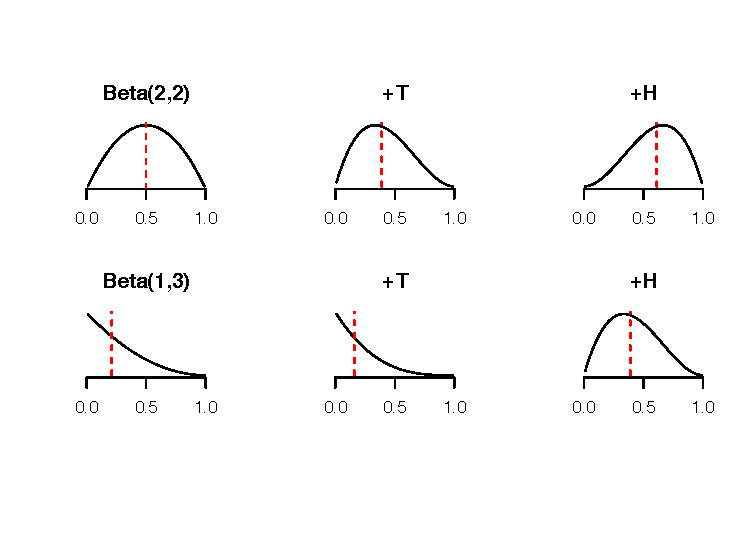
\includegraphics[width=3.25in]{figures/students2.pdf}
\end{center}
\vspace{-2ex}
\caption{\label{fig:students} Two examples of Beta distributions---representing individual students' posterior distributions over a target concept---with different priors and patterns of evidence. Black curves show the probability distribution with a given prior (left column) and after observing a single tail or head (middle and right columns). Red lines show the posterior mean.}
\vspace{-2ex}
\end{figure}

Students are modeled as Bayesian (optimal) estimators of the target Bernoulli parameter, using a conjugate Beta-Bernoulli distribution. This model is very convenient: The form of the prior distribution is $Beta(\alpha,\beta)$, and the form of the posterior can be written $Beta(\alpha+x,\beta+y)$ where $x$ and $y$ represent the number of heads (1s) and tails (0s) observed in the data. In this sense, if $x$ and $y$ are the \emph{counts} of observed data, then $\alpha$ and $\beta$ can be referred to as \emph{pseudo-counts}.

This formulation also gives us a way to model both the students' abilities and their prior knowledge about the situation. Consider the example distributions shown in Figure \ref{fig:students}. Symmetric priors of $\alpha=\beta=2$ lead to a bias that the $C$ is around .5, while $\alpha=1, \beta=3$ leads to a bias towards lower values of $C$. 

Under this formulation, the prior controls both the speed at which a student will learn and their overall bias. For example, as $\alpha$ and $\beta$ both go towards 0, the student's estimate converges to a maximum-likelihood estimate based on the observed data alone. In contrast, as $\alpha$ and $\beta$ both get larger, the student makes less and less use of the data and is more and more reliant on the shape of the prior distribution. The relative weights of $\alpha$ and $\beta$ control the student's mean estimate---greater pseudo-counts on one or the other will lead to greater bias to believe that the correct parameter is lower or higher. 

As described below, given our evaluation metric, students' learning rate is less important than their bias. For this reason, we use an alternative parameterization of the Beta-Bernoulli distribution, in terms of shape $\mu$ and scale $\nu$, where

\begin{eqnarray}
\mu &=&  \alpha / (\alpha + \beta) \\
\nu &=& \alpha + \beta
\end{eqnarray}

\noindent In this parameterization, $\mu$ directly controls the mean of the distribution, while $\nu$ captures the strength of the belief. For example, in Figure \ref{fig:students}, $\mu=.5$ for the top distribution and .25 for the bottom, while $\nu=4$ for both.

\subsection{Evaluation}

We compute the information gain for each student due to the teacher's chosen example. We notate the Beta distribution of the teacher's beliefs as $B_T = Beta(\alpha_T,\beta_T)$, and similarly the student's Beta distributions before and after seeing the teacher's example as $B_{S}$ and $B_{S+e}$ respectively. This allows us to compute the Kullback-Leibler divergence \cite{cover2012} between teacher and student, both before and after seeing example $e$. The KL divergence gives a measure of the distance between the true distribution $B_T$ and the approximations $B_{S}$ and $B_{S+e}$.
The difference between these two divergences gives the number of bits of information gained due to the example, which we refer to as ``information gain'':\footnote{I use this label for convenience, though note that this measure is not equivalent to mutual information, an information-theoretic quantity that is also occasionally referred to as ``information gain.''}

% LONG : rename so that it's not IG, which is not MI 

\begin{equation}
\label{eq:ig}
IG(e) = D_{KL} ( B_T || B_{S} )  - D_{KL} (B_T ||B_{S+e} ) 
\end{equation}

\noindent where the divergence measure is computed in closed form for e.g., $B_T$ and $B_S$, as

\begin{equation}
\label{eq:dkl}
\begin{split}
D_{KL} (B_T ||B_{S} )  = & \log( \frac{B(\alpha_{S},\beta_{S})}{B(\alpha_{T},\beta_{T})}) + \\
& (\alpha_T - \alpha_S) \psi (\alpha_T) + \\ 
& (\beta_T - \beta_S) \psi (\beta_T) + \\
& (\alpha_T - \alpha_S + \beta_T - \beta_S) \psi (\alpha_T + \beta_T). \\
\end{split}
\end{equation}

\noindent where $\psi$ denotes the digamma function and $B(a,b)$ denotes the beta function. Information gain will be positive when $B_{S+e}$ is closer to the target distribution than $B_S$. For purposes of comparison, we always consider information gain on a per-student basis. 

An interesting property of information gain defined in this way is that it is insensitive to the scale $\nu$ of the students' prior estimate and sensitive only to the shape $\mu$. If Equation \ref{eq:dkl} is substituted into Equation \ref{eq:ig}, and we assume that $e=1$, Equation \ref{eq:ig} reduces to\footnote{Full derivation is available in the github repository linked above.} 

\begin{equation}
IG(e) = \log(\frac{\alpha_S + \beta_S}{\alpha_S}) + \psi (\alpha_T) + \psi (\alpha_T + \beta_T).
\end{equation}

\noindent Only the first of these terms depends at all on the student's knowledge. That term ($\log(\frac{\alpha_S + \beta_S}{\alpha_S})$) depends on the ratio of $\alpha_S$ to $\beta_S$ but not their absolute values. Thus, only the relative size of $\alpha$ and $\beta$---captured via the $\mu$ parameter---matters. (The same result holds for $e=0$). Intuitively, this result implies that in the current setup a well-chosen example can always teach you more, and the amount it can teach you is related to the distance between your best estimate and that of the teacher. In addition, practically speaking, this result is convenient because we need only vary the $\mu$ parameter for individual students in our simulations and can hold $\nu$ constant.

\subsection{Teacher}

The teacher is assumed to choose between possible examples or sequences of examples in $E$. In the current simple case, $E=\{H,T\}$. This choice is made so as to maximize the average information gain across students. Thus, expected information gain is the information gain due to the best example that they could show:

\begin{equation}
E[IG] = \argmax_e {IG(e)}.
\end{equation}

\noindent Note that this formulation assumes that teachers have perfect knowledge of the students both before and after an example and can mentally simulate the effects of a particular example on student knowledge so as to pick the appropriate one. 

 \section{Simulations}
% \section{Simulations 1: Initial Results}

\begin{figure}[t]
\begin{center}
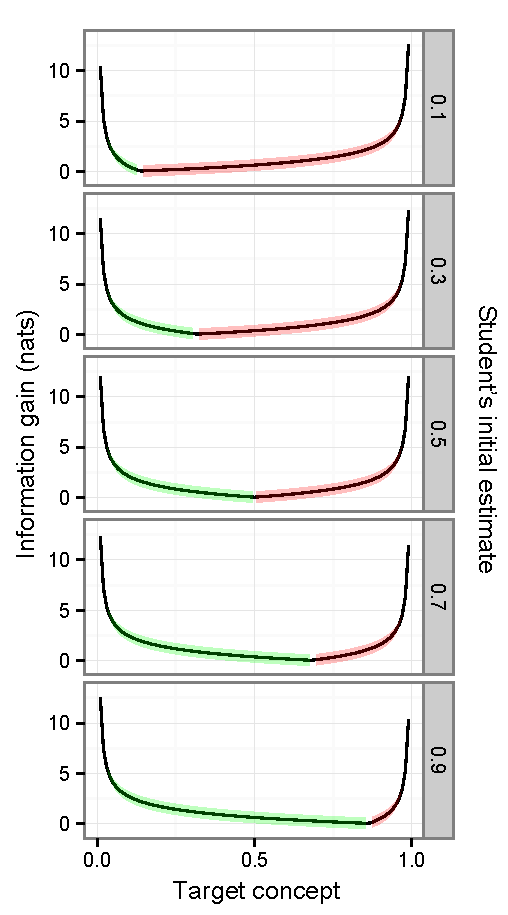
\includegraphics[width=2.25in]{figures/single_student_gain.pdf}
\end{center}
\vspace{-2ex}
\caption{\label{fig:student} Student's expected information gain, plotted by target concept $C$, for students with a range of different initial values of student's initial bias $\mu$ (panels). Green highlighting shows ranges in which the teacher's best move is providing $T$ (0), while red highlighting shows the range where $H$ (1) produces greater gain.}
\vspace{-2ex}
\end{figure}

The following sections report simulations using the model above, beginning with results for a single student (providing initial model validation). The next set of simulations show expected information gain for students based on the variance across students in a classroom and based on the size of the classroom. The last two simulations consider the function of ``differentiation'' (grouping students by their initial knowledge) and the problems that can arise for a mis-classified student. 

Apart from the initial simulation, for which results are computed analytically, all others use 1000 simulated classrooms per parameter setting, with students' $\mu$ values randomly generated from a Beta distribution for each simulation.

\subsection{Teaching a Single Student}



In the first simulation, I examine the teacher's optimal strategy (and information gain) for a single student. I generated students with initial biases $\mu= \{.1, .3, .5, .7, .9\}$, and varied the teacher's target concept $C$ smoothly. For each combination of $\mu$ and $C$, I assumed that the teacher chose the better of the two possible examples ($H$ or $T$). 

Results are shown in Figure \ref{fig:student}. Following intuitions, information gain is greatest when the teacher's concept is extreme, and when the student's initial expectation is mismatched to that concept. In addition, the teacher's optimal strategy (shown by the red or green ribbon) changes depending on the student's initial expectation. Consider the top panel: When the student starts out believing $C=.1$, the teacher should almost always select $H$ as his example, though the relative information gain can be low if the disparity between the student's belief and the teacher's is not large (e.g. if $C=.2$). Note also that information gain can be very slightly negative in the case that the student's belief exactly matches that of the teacher---given that match, any single example will move the student's belief further from that of the teacher. 

\subsection{Student Variability}

\begin{figure}[t]
\begin{center}
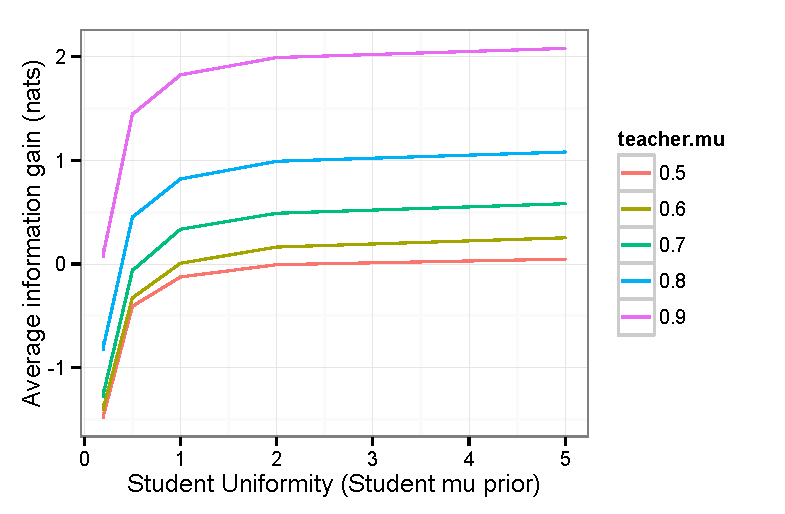
\includegraphics[width=3.5in]{figures/student_uniformity.pdf}
\end{center}
\vspace{-2ex}
\caption{\label{fig:uniformity} Information gain, plotted by the prior on students' uniformity (a symmetric Beta distribution from which each student's $\mu$ parameter is chosen). Target values for $C$ are shown in different colors. Error bars (in some cases invisible) show 95\% confidence intervals.}
\vspace{-2ex}
\end{figure}

The next set of simulations combines several students in a single classroom. In these and all subsequent simulations, I generated students randomly via a symmetric Beta prior distribution on student $\mu$ values. With $\alpha,\beta$ both $< 1$, this produces classrooms with students who have extremal biases (e.g. close to 0 and 1); with $\alpha,\beta>1$, this produces classrooms of students whose biases tend to be clustered closer and closer to .5. For each classroom, I assume that the teacher calculates her expected information gain for her two possible strategies and then uses the better of the two. 

Greater student uniformity produced greater information gain, for all target concepts. Figure \ref{fig:uniformity} shows this relationship. The effect was greatest for the smallest values, and information gain was very low when students' expectations tended to be extremal but the target value was closer to the middle of the range. 

For $\mu$ priors $< 1$ information gain can actually be negative; this result comes about when student expectations are extremal but the target value is moderate. In these cases, a single piece of evidence will either reinforce students' biases (in the case that their guess is already close to 1 and they see an $H$) or fail to counteract their biases (in the case that their guess is close to 0 and they again see a $H$). The average of these two cases is negative.

This simulation suggests that students in a more heterogenous classroom will learn less, on average, because the teacher will be less able to tailor her examples to the students' knowledge. In contrast, in a more homogeneous classroom, the teacher can better provide an example that leads to learning for all students. 

\subsection{Classroom Size}

\begin{figure}
\begin{center}
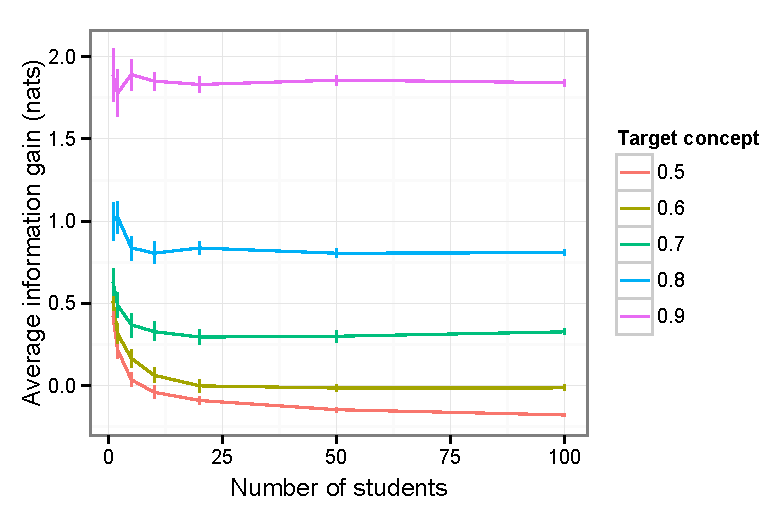
\includegraphics[width=3.5in]{figures/class_size.pdf}
\end{center}
\vspace{-2ex}
\caption{\label{fig:class} Average information gain plotted by number of students in a class. Target values for $C$ are shown in different colors. Error bars show 95\% confidence intervals.}
\vspace{-2ex}
\end{figure}


% run more simulations for smaller classes, because of small sample variability

\begin{figure*}
\begin{center}
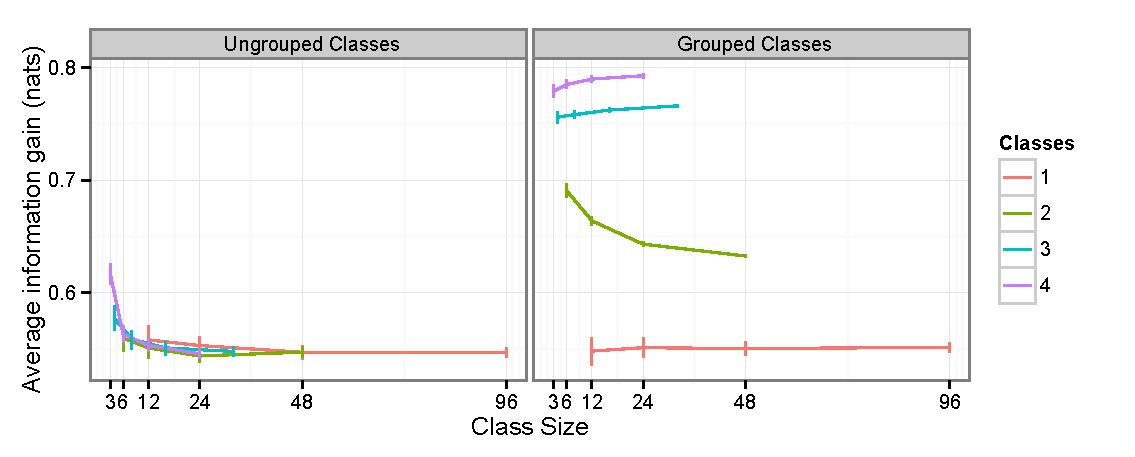
\includegraphics[width=5.5in]{figures/grouping.pdf}
\end{center}
\vspace{-2ex}
\caption{\label{fig:grouping} Information gain plotted by the number of students in a class. $C$ is set to .75 for illustrative purposes. Colors show the total number of classes among which students were distributed. In the left (ungrouped) panel, students were distributed at random; in the right (grouped) panel, students were sorted by their prior $\mu$ value. Error bars show 95\% confidence intervals.}
\vspace{-2ex}
\end{figure*}

The previous simulation set showed that, all else being equal, heterogeneity of students has a very negative effect on teachers' ability to chose strategies that lead to optimal information gain: More heterogeneous students provide the teacher less of a chance to customize the teaching environment to each student's knowledge state. An important corollary of this finding is that class size is an important factor influencing heterogeneity. Larger classes should be, on average, more heterogeneous, and should hence provide fewer opportunities for teachers to customize their message in ways that produce greater information gain.

I simulated classrooms from 1 -- 100 students, across a range of target values for $C$ and found precisely this effect: Larger classrooms showed less average information gain (Figure \ref{fig:class}). The  effect was substantially smaller in magnitude than the heterogeneity effects in the preceding simulations---class size acts only indirectly on variability. 

In addition, the class size effect varied substantially with $C$. Here is the intuition behind this result: If $C=.9$, nearly all students---regardless of how many there are---will gain information if the teacher presents a 1. In contrast, if $C=.5$, on average about half of the students in each class begin with a value of $\mu < .5$, and the other half begin believing $\mu > .5$. But if the class average is actually $.5$ then there is no teaching opportunity. It is only if the class average is (say) $.6$ that the teacher can pull it back down towards $.5$ by presenting a 0. As class size increases, student means tend to cancel each other out and  on average no individual example will teach the class anything. 

Overall, this simulation suggests that class size exerts a negative effect on performance, especially for tricky concepts where students' initial starting points vary meaningfully. 

\subsection{Grouping Students by Knowledge or Ability}


%% could try redoing this by number of tracks, rather than class size (on the x)

One way to mitigate class size effects is by reducing heterogeneity either in classrooms as a whole or in the instruction of individual topics. This reduction is sometimes achieved via what is known as ``tracking''---assigning students to classrooms systematically by knowledge or ability, rather than assigning them randomly---and sometimes via ``differentiation,'' where the instruction of individual topics is tailored to individual groups. The next simulations examine the effects of grouping on performance.\footnote{I refer to this broader set of strategies as ``grouping'' strategies because our current model does not allow for a difference between grouping at the level of individual lessons (``differentiation'') vs. classroom assignment (``tracking'').} 

I created two parallel sets of classrooms. In each, a population of students was generated with uniform bias values. The ungrouped simulations were identical to the class-size simulations above; the grouped simulations were identical except that students were sorted and distributed into available classes based on their $\mu$ value. For example, if there were two classes, the first would receive the students with values of $\mu$ below the median. 

Grouping resulted in greater average information gain for students. Results for an example value of $C$ are shown in Figure \ref{fig:grouping}. While the ungrouped classes were not differentiated from one another and showed a small class-size effect (left panel), the grouped classes showed greater information gain as the number of subgroups of students increased. Interestingly, the advantage decreased with each additional group---too many groups created diminishing returns \cite{tomlinson1999}. There was no class-size effect for the simulations with 3 and 4 groups: Performance remained stable as size increased, presumably because the classes were homogeneous enough that additional students did not make an appreciable difference to outcomes.  

Class size was a negative predictor of student learning because of the relationship between classroom heterogeneity and student learning. Larger classes tend to be more heterogeneous and hence to have lower performance, but grouping students by prior bias reduced this effect.

\subsection{Mis-assignment for an Individual Student}

\begin{figure}
\begin{center}
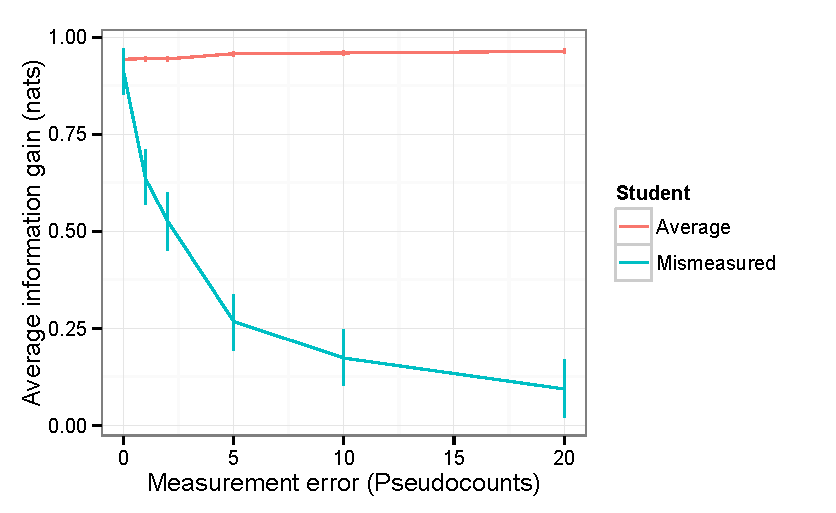
\includegraphics[width=3.5in]{figures/mismeasured.pdf}
\end{center}
\vspace{-2ex}
\caption{\label{fig:mismeasure} Information gain for the average student (red) and a student whose parameters have been mismeasured (blue), plotted by the error in the measurement. Simulation data are shown for $C=.75$ with four tracked classes of 24 students each. Error bars show 95\% confidence intervals.}
\vspace{-2ex}
\end{figure}

What happens if you are grouped with the wrong set of students? The last simulation explores the measurement of individual students' competence in the grouping scenario described above. 

The base scenario for these simulations is a group of 96 students grouped into four classes (as shown in Figure \ref{fig:grouping}). I altered this simulation by assuming that the teacher's knowledge of one student's $\mu$ value was perturbed by a known number of pseudocounts, varying from 0--20. The result of this perturbation was that this student was likely to be assigned to a mismatched classroom. Average information gain for the mis-assigned student declined substantially with even relatively small perturbations (Figure \ref{fig:mismeasure}). This simulation suggests that, even within the restricted world of the model, mismeasurement or misassignment of a student has substantial consequences for learning.

\section{Discussion}

Based on the idea that a good teacher is a good communicator, this paper proposed a model of classroom teaching. The model describes teachers as choosing optimal messages to alter student's beliefs about a target concept, where optimal messages are those that maximize the average information gain across students in the classroom. Simulations show that several results follow naturally from this construal of teaching. First, classroom heterogeneity substantially limits the teacher's ability to choose appropriate examples to change students' beliefs. Because of this fact about the model and the idiosyncrasies of small samples of students, smaller classrooms tend to lead to better learning. In addition, grouping students to reduce variability led to substantial increases in information gain (though these depended on accurate classification of students). The model presented here thus provides a first attempt at a generative framework for the dynamics of classroom education. 

In the current model, the teaching game---presenting coin flips to estimate the coin's weight---is exceedingly simple; this simplicity is both a strength and a limitation of the current work. By using the conjugate model chosen here, many parts of choosing an optimal strategy became computationally tractable; in addition, this particular model allowed an analytic reduction in the parameter space, vastly facilitating the project of characterizing its dynamics. Nevertheless, a necessary direction for future work is to test the generality of the findings reported here with another learning model; a clear candidate would be the concept-learning tasks studied by \citeA{shafto2008}. 

More broadly, the current model incorporates a large number of optimality assumptions, prominently including 1) optimal strategy choice by teachers, 2) optimal teacher knowledge of students, and 3) optimal learning by those students. Relaxing any one of these would lead to interesting future investigations, of 1) heuristic strategy choice, 2) consequences of noisy teacher assessments of student knowledge, or 3) strategies for coping with a wider range of students (respectively). Such extensions might reveal connections with other areas of educational interest (e.g. formative student assessment; \citeNP{torrance1998}). 

More broadly, the suggestion of the current work is that models of pragmatic communication may have a place in understanding classroom teaching. The challenge for such models in the future will be enriching them until they are able to make direct contact with empirical data. 

\section{Acknowledgments}

Many thanks to Noah Goodman, Roger Levy, Long Ouyang, and Chris Potts for valuable discussion.

\bibliographystyle{apacite}

\setlength{\bibleftmargin}{.125in}
\setlength{\bibindent}{-\bibleftmargin}

\bibliography{teaching}


\end{document}
